\documentclass{TDP003mall}



\newcommand{\version}{Version 1.1}
\author{Nils Bark, \url{nilba048@student.liu.se}\\
  Hadi Ansari, \url{hadan326@student.liu.se}}
\title{Systemdokumentation}
\date{2020-10-20}
\rhead{Nils Bark\\
Hadi Ansari}


\begin{document}
\projectpage
\section{Revisionshistorik}
\begin{table}[!h]
\begin{tabularx}{\linewidth}{|l|X|l|}
\hline
Ver. & Revisionsbeskrivning & Datum \\\hline
1.1 & Andra versionen av systemdokumentation skapad enligt komplettering & 2020-10-20 \\\hline
1.0 & Första versionen av systemdokumentation skapad & 2020-10-15 \\\hline
\end{tabularx}
\end{table}

\section{Översikt}
\begin{figure}[h!]
  \centering
  \includegraphics[scale=0.5]{översikt.jpg}
  \label{Bild 1}
  \caption{Hur projektets delar samspelar.}
\end{figure}
Portfolion består i grunden av två lager: Datalagret, som hämtar och sorterar data om projekt från en JSON-fil. Det består av filerna data.py och data.json.
Det andra lagret är presentationslagret, som tar in datan från datalagret och sedan presenterar den med hjälp av flera mallar. Det består av myFlaskProject.py
, stylesheet.css, mallarna under templates/ och bilderna under static/images/. En översiktlig bild över hur delarna samspelar finns ovan (figur 1) som visar hur
datalagret (med hjälp av db) och presentationslagret plus Jinja kommunicerar för att visa resultatet i HTML och CSS .


\section{Felhantering}
För de fel som enligt testningen riskerar att uppstå under vanligt användande finns specifika sidor med felmeddelanden redo att presenteras för användaren.
Till exempel visas en sida med ``Projektet du försöker nå finns inte'' om project() får ett projekt-ID som inte finns i databasen. Även HTTP felkoder som
404 och 500 hanteras. För en detaljerad översikt över alla HTTP meddelanden som kan dyka upp bör man titta i terminalen medan hemsidan är aktiv.

Felsökning sker mestadels genom att testa webbsidan live i webbläsaren och genom att titta i koden. Även det gemensamma testprogrammet data\_test.py användes
regelbundet under projektets gång.
\section{Datalagret}
Detta delsystem har ansvar för datan som står i databasen. Den erbjuder funktionalitet som efterfrågas från presentationslagret. Datalagret och dess funktioner
är utformade efter de krav som finns i specifikationerna på kursens hemsida. I projektet används alla dessa funktioner förutom \textit{get\_techniques()} och
\textit{get\_technique\_stats()}. Data-modulen importeras i presentations-modulen för att erbjuda dessa funktioner när det behövs. Nedan ges en kort beskrivning kring hur funktionerna används i presentations-modulen:
\begin{itemize}
\item \textit{load()}: Används för att ladda projeken från databasen
\item \textit{search()}: Används på flera ställen i presentations-modulen men generellt sett används när en sökning ska utföras.
\item \textit{get\_project()}: Används för att returnera ett specifikt projekt som matchar id:t. 
 \end{itemize}

\section{Presentationslagret}
Presentationslagret har hand om inmatning från användaren. Det kan med hjälp av denna information anropa på lämpliga funktioner från datalagret för att sedan visa
passande resultat. Den använder sig av Jinja för att tolka Html mallar och skapa relevanta webbsidor.
Nedan beskrivs alla funktioner som ingår i presentationslagret tillsammans med sekvensdiagram för de fyra funktionerna som står för projektets fyra sidor.

\subsection{load\_db()}
Kallar på load-funktionen från datalagret för att ladda datan från JSON-filen. Upprepas i funktionerna som laddar olika sidor så att de kan reflektera ändringar i JSON-filen
direkt. Anledningen till att det finns en \textit{load\_db()} funktion i presentationslagret är för att slippa anropa \textit{load(``Data.json'')} på flera ställen i presentationslagret.
Den anropas inuti \textit{load\_db()} på ett och samma ställe och på så sätt kan det bli enklare att byta ``data.json'' om sådant behövs senare i framtiden. Nedan finns en bild som
visar hur \textit{load\_db()} är uppbyggd:



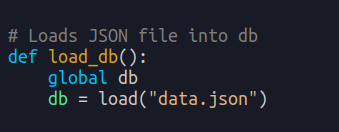
\includegraphics[scale=0.5]{Images/load_db.png}

\subsubsection*{Returnerar: lista}
Returnerar en lista med dictionaries som innehåller projektdatan från JSON-filen.


\newpage
\subsection{index()}
Laddar portfolions startsida och hämtar de tre senaste projekten (baserat på slutdatum) från databasen. Eftersom startsidan är en dynamisk sida uppdateras den genom ett GET request
utan att den behöver inmatning från användaren.
\subsubsection*{Returnerar: HTML-fil}
HTML-fil baserad på mallen ``index.html'' och resulterande projektlista som kan nås på ``URL: /''. 
\subsubsection*{Sekvensdiagram}
Nedan i figur 2 visas funktionaliteten för index i mer detalj.
\begin{figure}[!h]
  \centering
  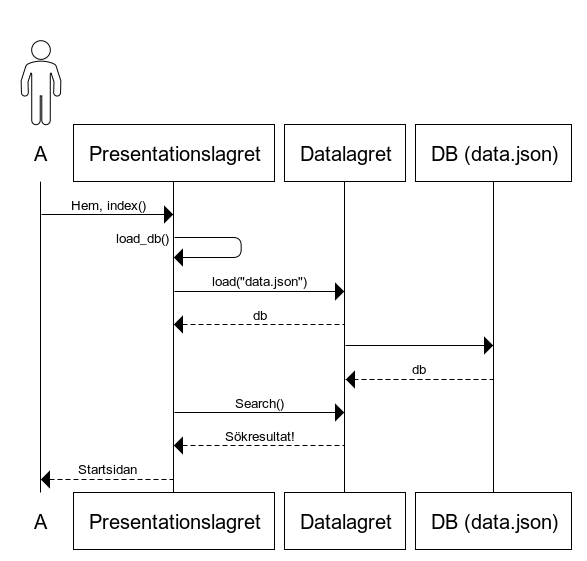
\includegraphics[scale=0.5]{index.png}
  \label{Bild 2}
  \caption{Sekvensdiagram för sidan index.html}
\end{figure}

\newpage
\subsection{project\_list()}
Hämtar användarens inmatning med hjälp av ett GET request och presenterar matchande projekt från databasen i form av en lista baserat på den. Om ingen inmatning finns
presenteras alla objekt sorterade efter namn.
\subsubsection*{Returnerar: HTML-fil}
HTML-fil baserad på mallen ``project\_list.html'' och angiven sökdata. Resulterande projektlista kan nås på ``URL: /list''. 
\subsubsection*{Sekvensdiagram}
Nedan i figur 3 visas funktionaliteten för project\_list i mer detalj.
\begin{figure}[!h]
  \centering
  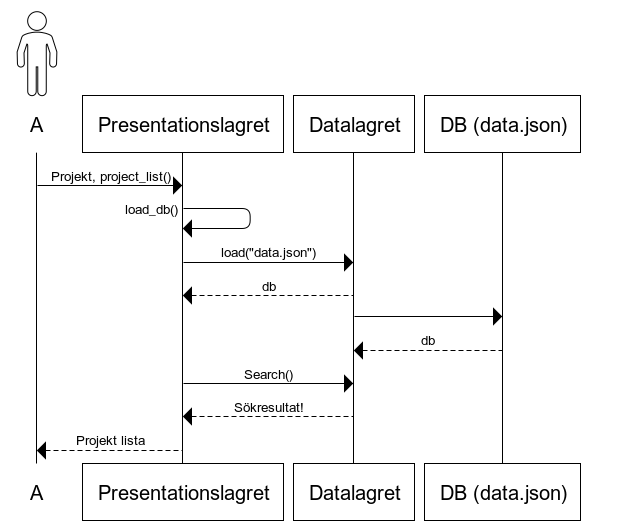
\includegraphics[scale=0.5]{projekt_lista.png}
  \label{Bild 3}
  \caption{Sekvensdiagram för sidan project\_list.html}
\end{figure}

\newpage
\subsection{project(id)}
Laddar en sida baserad på det angivna ID:t då det matchas mot tillgängliga ID:n i databasen med hjälp av ett GET request. Ger ett felmeddelande i form av en annan sida ifall ID:t är ogiltligt.
\subsubsection*{Parametrar}
\begin{itemize}
\item \textbf{id:} ID för projektet som ska kallas på.
\end{itemize}
\subsubsection*{Returnerar: HTML-fil}
HTML-fil baserad på mallen ``project.html'' och angivet projekt-ID. Resultatet kan nås på ``URL:/project/id''.
\subsubsection*{Sekvensdiagram}
Nedan i figur 4 visas funktionaliteten för project(id) i mer detalj.
\begin{figure}[!h]
  \centering
  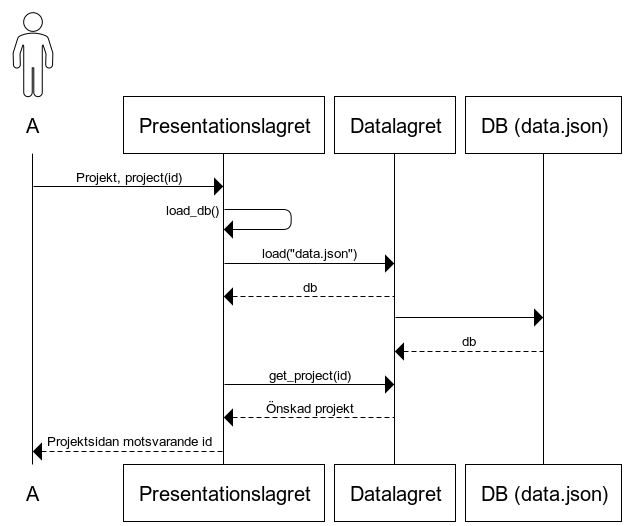
\includegraphics[scale=0.5]{projekt.png}
  \label{Bild 4}
  \caption{Sekvensdiagram för sidan project.html}
\end{figure}


\newpage
\subsection{techniques()}
Tar användarens inmatning (endast i form av tekniker) med hjälp av ett GET request och presenterar matchande projekt från databasen i form av en lista. Utan inmatning
visas alla projekt sorterade efter namn.
\subsubsection*{Returnerar: HTML-fil}
HTML-fil baserad på mallen ``techniques.html'' och angiven sökdata. Resulterande sidan kan nås på ``URL:/techniques''.
\subsubsection*{Sekvensdiagram}
Nedan i figur 5 visas funktionaliteten för techniques i mer detalj.
\begin{figure}[!h]
  \centering
  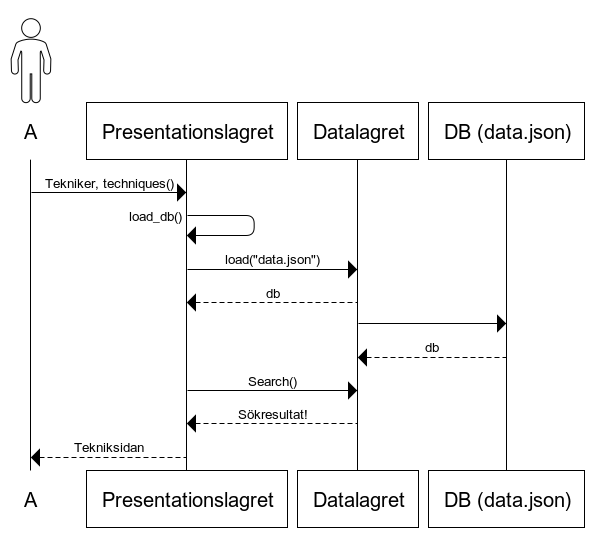
\includegraphics[scale=0.5]{tekniker.png}
  \label{Bild 5}
  \caption{Sekvensdiagram för sidan techniques.html}
\end{figure}

\end{document}
